%*******10********20********30********40********50********60********70********80
\clearpage
\subsection{Aggregate Ratio Related to Behavior of Concrete During DEF Expansion}
% A15X0Cfix vs A15X0Cfix
In this section, the relationship between aggregate ratio and behavior during expansion is discussed.

Expansion simulation result between 15\% coarse aggregate model and 30\% coarse aggregate model is compared here to analysis how the change in aggregate percentage influence the cracking pattern in different expansion ratio.

\begin{figure}[!h]
\centering
\begin{subfigure}{.5\textwidth}
  \centering
  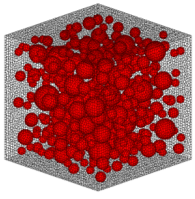
\includegraphics[width=.4\linewidth]{Files/Aggregate/A15.png}
  \caption{15\% Coarse Aggregate}
  \label{fig:A15_model}
\end{subfigure}%
\begin{subfigure}{.5\textwidth}
  \centering
  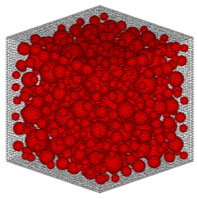
\includegraphics[width=.4\linewidth]{Files/Aggregate/A30.png}
  \caption{30\% Coarse Aggregate}
  \label{fig:A15_model}
\end{subfigure}
\caption{Coarse Aggregate Percentage}
\label{fig:Aggregate_Percentage}
\end{figure}


From Table \ref{table:DEF_15vs30_EXP} can be seen that with same expansion step and same initial strain given in each step, the global expansion of with less coarse aggregate (A15 cases here) is higher than less coarse aggregate cases (A30 cases here).  As coarse aggregate ratio increased, DEF reactive interfaces decrease, which suggested the reason for achieving smaller global expansion in higher coarse aggregate cases.

\begin{table}[ht!]
\centering
\begin{tabular}{ ||p{2cm}|p{2cm}|p{2cm}|p{2cm}|| }
 \hline
    Initial Strain (Each Step) & Expanding Steps & A15 Final Expansion & A30 Final Expansion[\%] \\ [0.5ex]
 \hline\hline
  0 & 0 & 0 & 0 \\
  0.001 & 20 & 0.1645 & 0.1379\\
  0.002 & 20 & 0.3413 & 0.2873\\
  0.004 & 20 & 0.6631 & 0.5795\\
  0.006 & 20 & 0.9587 & 0.8785\\
 \hline
\end{tabular}
\caption{One Dimensional Expansion Ratio in Single DEF Model Simulation}
\label{table:DEF_15vs30_EXP}
\end{table}

\begin{figure}[ht!]
\centering
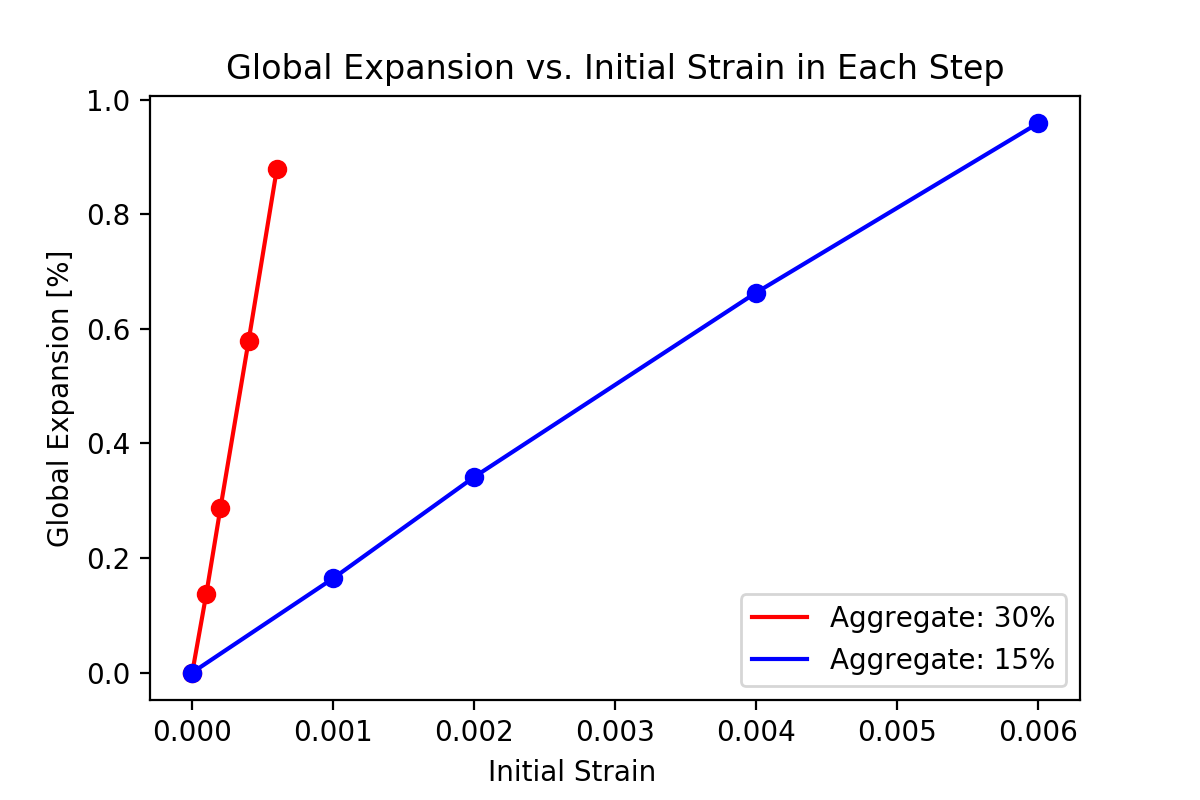
\includegraphics[width=.8\linewidth]{Files/exp_plot/DEFA30vsA15_exp.png}
  \caption{Global Expansion vs. Step}
  \label{fig:DEFA30vsA15_exp}
\end{figure}

\begin{figure}[!h]
\centering

    %*******
    \begin{subfigure}{.5\textwidth}
      \centering
      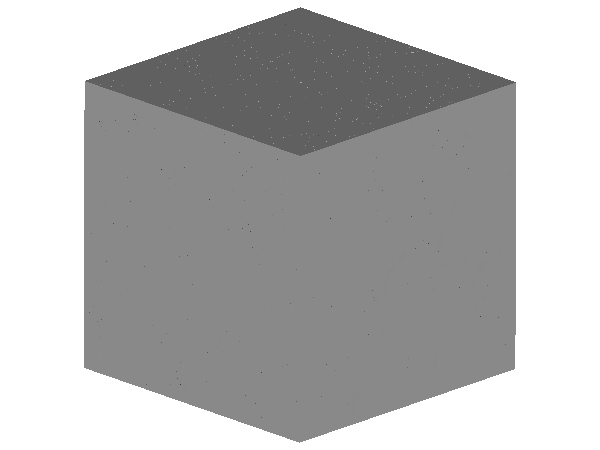
\includegraphics[width=.8\linewidth]{Files/exp_3D/ASR/A30Undamaged.png} %TODO: Fix. Should be A15
    \caption{Case 0: 0\% Expansion}
    \end{subfigure}%
    %*******
    \begin{subfigure}{.5\textwidth}
      \centering
      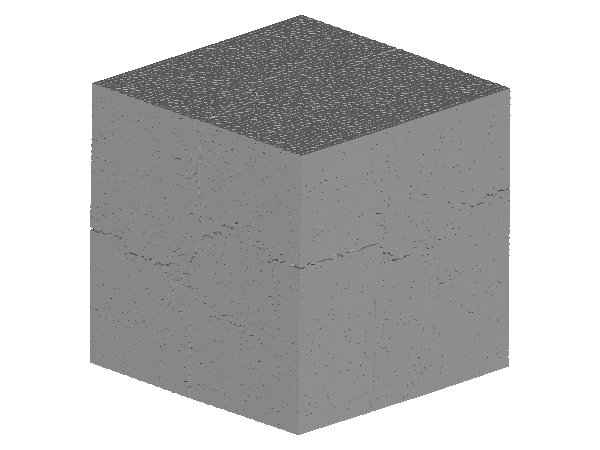
\includegraphics[width=.8\linewidth]{Files/exp_3D/DEF/A15X0C_1_3d.png}
    \caption{Case 1: 0.1645\% Expansion}
    \end{subfigure}
    %*******
    \begin{subfigure}{.5\textwidth}
      \centering
      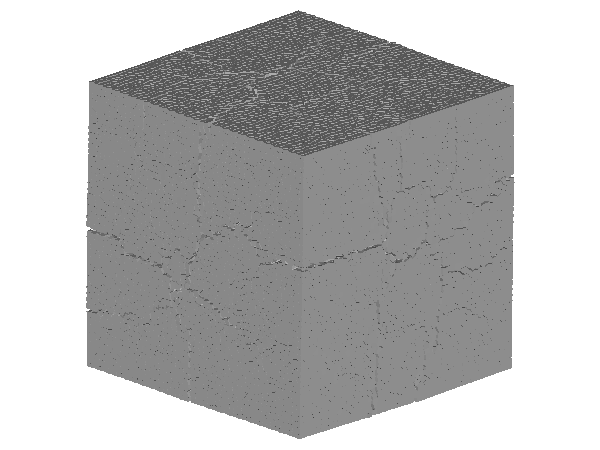
\includegraphics[width=.8\linewidth]{Files/exp_3D/DEF/A15X0C_2_3d.png}
    \caption{Case 2: 0.3413\% Expansion}
    \end{subfigure}%
    %*******
    \begin{subfigure}{.5\textwidth}
      \centering
      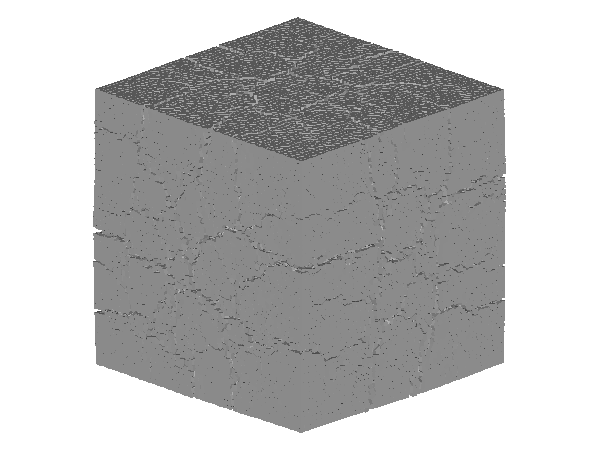
\includegraphics[width=.8\linewidth]{Files/exp_3D/DEF/A15X0C_3_3d.png}
    \caption{Case 3: 0.6631\% Expansion}
    \end{subfigure}
    %*******
    \begin{subfigure}{.5\textwidth}
      \centering
      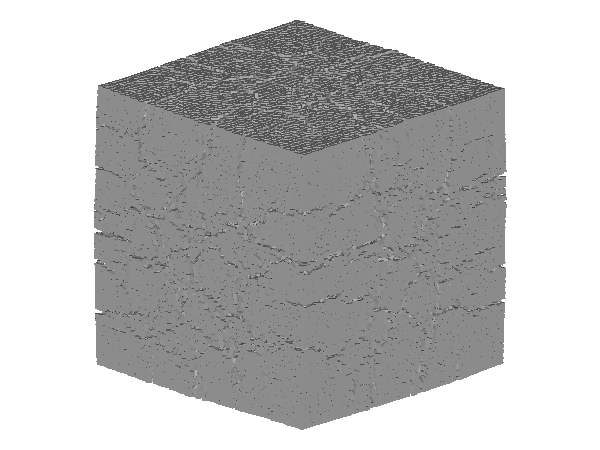
\includegraphics[width=.8\linewidth]{Files/exp_3D/DEF/A15X0C_4_3d.png}
    \caption{Case 4: 0.9587\% Expansion}
    \end{subfigure}%
    %*******

  \caption{3D Surface Cracks}
  \label{fig:DEF_A15X0C_3D}
\end{figure}

% Surface of one side
\begin{figure}[!h]
\centering

    %*******
    \begin{subfigure}{.5\textwidth}
      \centering
      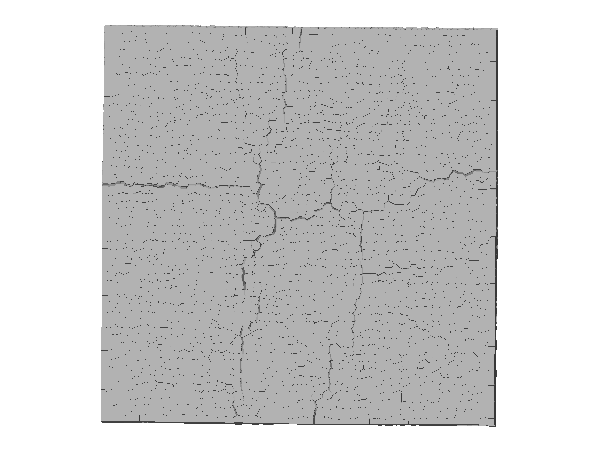
\includegraphics[width=.8\linewidth]{Files/exp_3D/DEF/A15X0C_1_3ds.png}
    \caption{Case 0: 0\% Expansion}
    \end{subfigure}%
    %*******
    \begin{subfigure}{.5\textwidth}
      \centering
      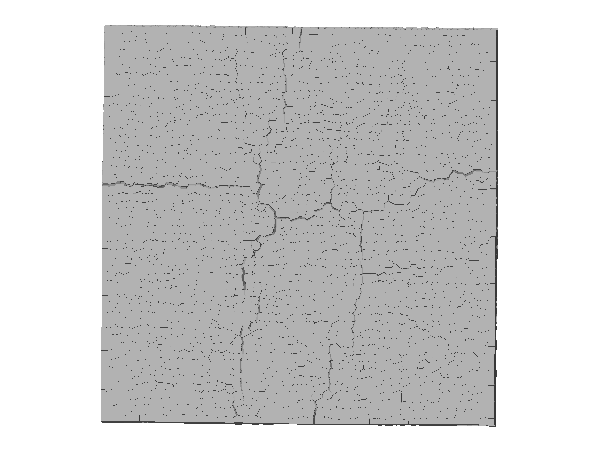
\includegraphics[width=.8\linewidth]{Files/exp_3D/DEF/A15X0C_1_3ds.png}
    \caption{Case 1: 0.1645\% Expansion}
    \end{subfigure}
    %*******
    \begin{subfigure}{.5\textwidth}
      \centering
      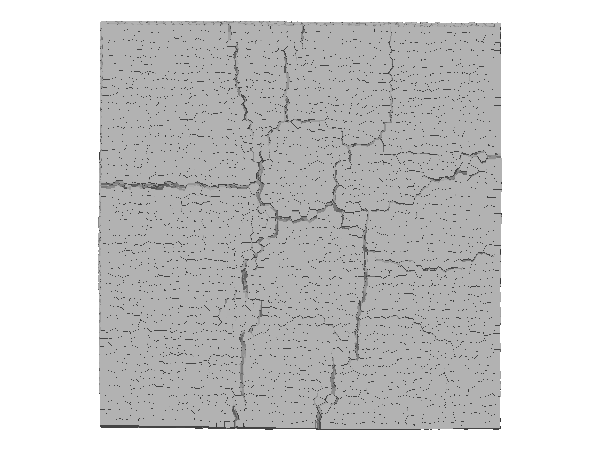
\includegraphics[width=.8\linewidth]{Files/exp_3D/DEF/A15X0C_2_3ds.png}
    \caption{Case 2: 0.3413\% Expansion}
    \end{subfigure}%
    %*******
    \begin{subfigure}{.5\textwidth}
      \centering
      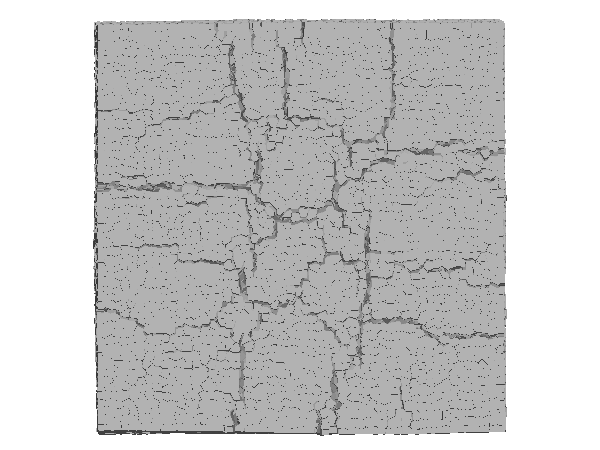
\includegraphics[width=.8\linewidth]{Files/exp_3D/DEF/A15X0C_3_3ds.png}
    \caption{Case 3: 0.6631\% Expansion}
    \end{subfigure}
    %*******
    \begin{subfigure}{.5\textwidth}
      \centering
      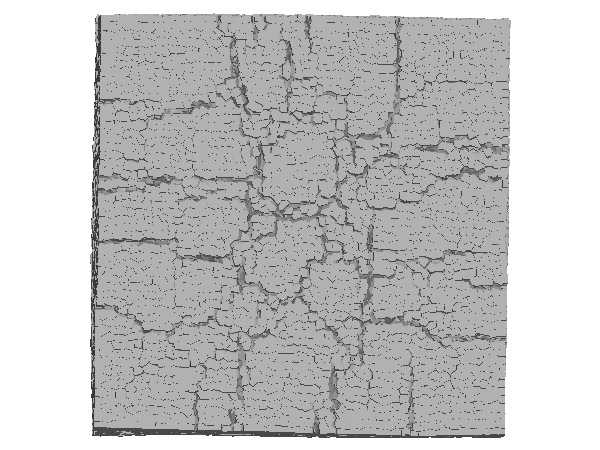
\includegraphics[width=.8\linewidth]{Files/exp_3D/DEF/A15X0C_4_3ds.png}
    \caption{Case 4: 0.9587\% Expansion}
    \end{subfigure}%

  \caption{3D Surface Cracks (Single Side View)}
  \label{fig:ASR_A15X0C_3DS}
\end{figure}

% Surface of one side
\begin{figure}[!h]
\centering

    %*******
    \begin{subfigure}{.5\textwidth}
      \centering
      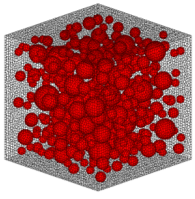
\includegraphics[width=.6\linewidth]{Files/Aggregate/A15.png}
    \caption{Case 0: 0\% Expansion}
    \end{subfigure}%
    %*******
    \begin{subfigure}{.5\textwidth}
      \centering
      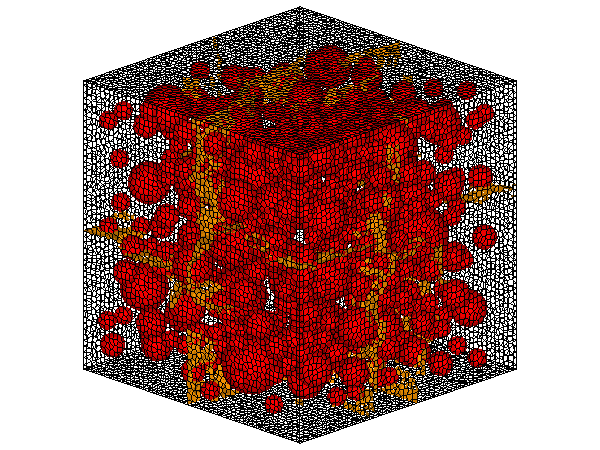
\includegraphics[width=.8\linewidth]{Files/exp_3D/DEF/A15X0C_1_c.png}
    \caption{Case 1: 0.1645\% Expansion}
    \end{subfigure}
    %*******
    \begin{subfigure}{.5\textwidth}
      \centering
      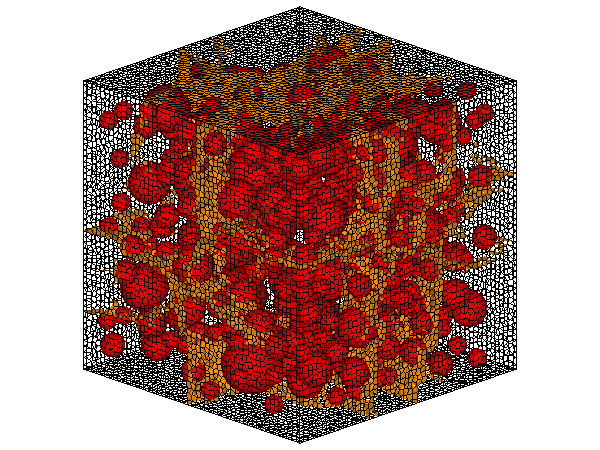
\includegraphics[width=.8\linewidth]{Files/exp_3D/DEF/A15X0C_2_c.png}
    \caption{Case 2: 0.3413\% Expansion}
    \end{subfigure}%
    %*******
    \begin{subfigure}{.5\textwidth}
      \centering
      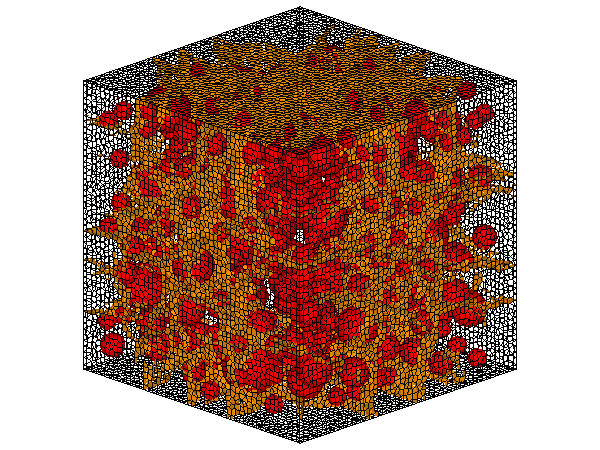
\includegraphics[width=.8\linewidth]{Files/exp_3D/DEF/A15X0C_3_c.png}
    \caption{Case 3: 0.6631\% Expansion}
    \end{subfigure}
    %*******
    \begin{subfigure}{.5\textwidth}
      \centering
      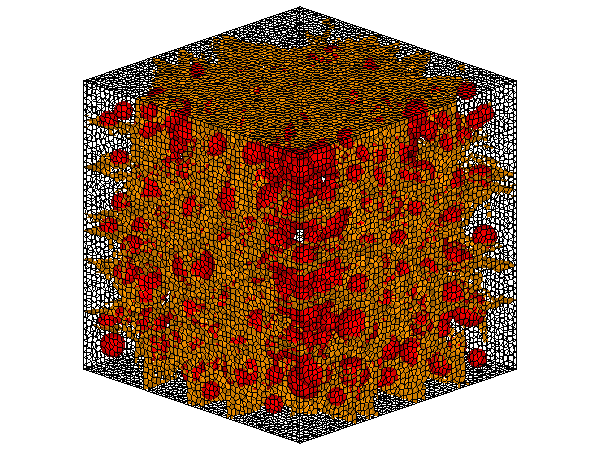
\includegraphics[width=.8\linewidth]{Files/exp_3D/DEF/A15X0C_4_c.png}
    \caption{Case 4: 0.9587\% Expansion}
    \end{subfigure}%

  \caption{3D Inner Cracks Larger than 0.03mm}
  \label{fig:ASR_A15X0C_crack}
\end{figure}

Figure \ref{fig:DEF_A15X0C_3D} and Figure \ref{fig:DEF_A15X0C_3DS} show surface crack pattern after DEF expansion of 15\% coarse aggregate cases.

Here 2 cases from 15\% coarse aggregate model and 30\% coarse aggregate model in relatively close global expansion rate are compared to show the influence of coarse aggregate ratio on cracking pattern.

For the aggregate ratio of 15\% model, case 3 is chosen, giving 0.0004mm initial strain for intensified DEF reactive interfaces, and reached 0.6631\% one-dimensional expansion after 20 steps. And for the aggregate ratio of 30\% model, case 3 is chosen, giving 0.004mm initial strain for DEF reactive interfaces and reached 0.5795\% one-dimensional expansion after 20 steps.

If plot the global expansion with initial strain given in each step to simulate DEF expansion, it can be seen that model with higher percentage of aggregate reach higher global expansion in the same initial strain giving comparing to to lower aggregate content one. %FIXME: WHY?

This may caused by more complicated interaction between expanded pastes and aggregate.

\clearpage

\begin{figure}[ht!]
\centering

    %*******
    \begin{subfigure}{.5\textwidth}
      \centering
      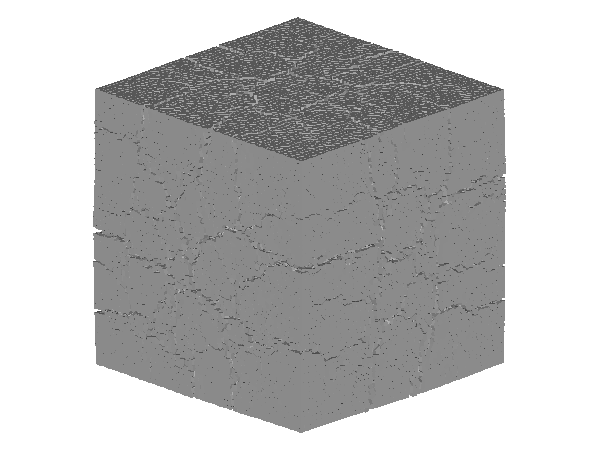
\includegraphics[width=.8\linewidth]{Files/exp_3D/DEF/A15X0C_3_3d.png}
    \caption{A15 Case 3: 0.6631\% Expansion \\ 3D Surface Crack}
    \end{subfigure}%
    %*******
    \begin{subfigure}{.5\textwidth}
      \centering
      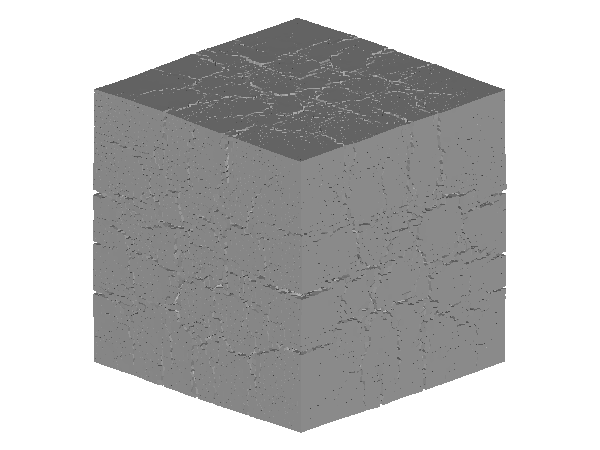
\includegraphics[width=.8\linewidth]{Files/exp_3D/DEF/A30X0C_3_3d.png}
    \caption{A30 Case 3: 0.4223\% Expansion\\ 3D Surface Crack}
    \end{subfigure}
    %*******
    \begin{subfigure}{.5\textwidth}
      \centering
      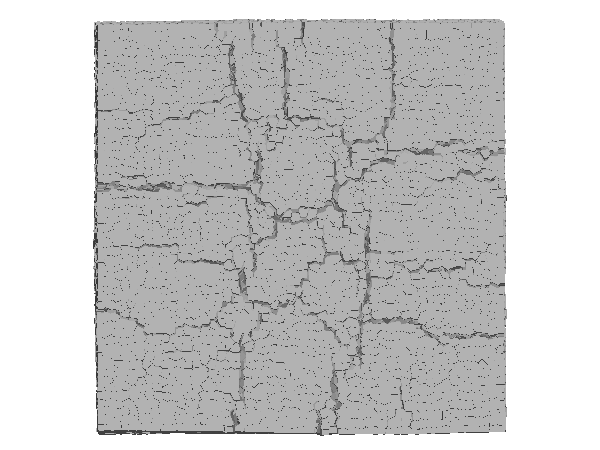
\includegraphics[width=.8\linewidth]{Files/exp_3D/DEF/A15X0C_3_3ds.png}
    \caption{A15 Case 3: 0.6631\% Expansion \\ 3D Surface Cracks (Single Side View)}
    \end{subfigure}%
    %*******
    \begin{subfigure}{.5\textwidth}
      \centering
      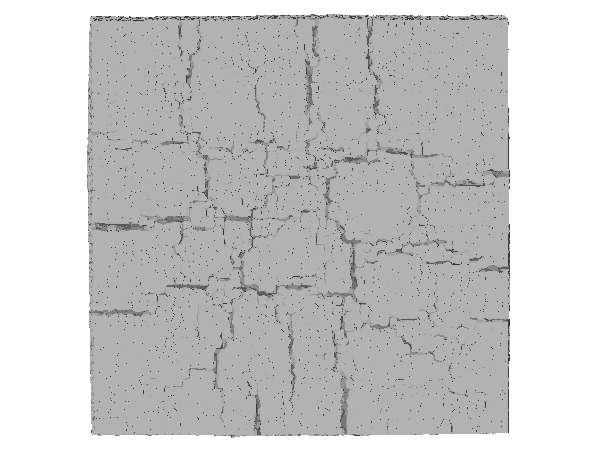
\includegraphics[width=.8\linewidth]{Files/exp_3D/DEF/A30X0C_3_3ds.png}
    \caption{A30 Case 3: 0.4223\% Expansion\\ 3D Surface Cracks (Single Side View)}
    \end{subfigure}
    %*******
    \begin{subfigure}{.5\textwidth}
      \centering
      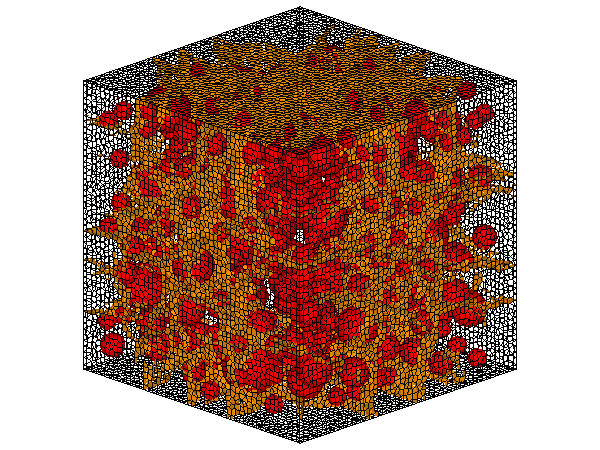
\includegraphics[width=.8\linewidth]{Files/exp_3D/DEF/A15X0C_3_c.png}
    \caption{A15 Case 3: 0.6631\% Expansion \\ 3D Surface Crack}
    \end{subfigure}%
    %*******
    \begin{subfigure}{.5\textwidth}
      \centering
      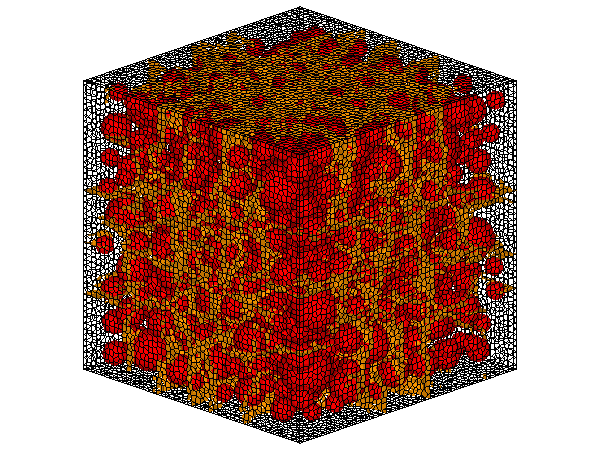
\includegraphics[width=.8\linewidth]{Files/exp_3D/DEF/A30X0C_3_c.png}
    \caption{A30 Case 3: 0.4223\% Expansion\\ 3D Surface Crack}
    \end{subfigure}
    %*******


  \caption{Comparing Between A15 and A30 3D Cracks}
  \label{fig:DEF_A15vsA30X0C_3D}
\end{figure}

\begin{table}[!h]
\centering
\begin{tabular}{ ||p{4cm}|p{4cm}|p{4cm}|| }
\hline
 Crack Width [mm] &  A15 Case 3 Total Cracked Interfaces &  A30 Case 3 Total Cracked Interfaces \\
 \hline\hline

   0.00000 - 0.00005 & 396456 & 367538 \\
   0.00005 - 0.00010 & 344516 & 328471 \\
   0.00010 - 0.00020 & 294996 & 294472 \\
   0.00020 - 0.00050 & 231816 & 251035 \\
   0.00050 - 0.00100 & 151693 & 186058 \\
   0.00100 - 0.00300 & 105939 & 133854 \\
   0.00300 - 0.01000 &  3983 &  57421\\
   0.01000 - 0.03000 & 696 & 1736 \\
   0.03000 - 0.10000 & 0 & 0 \\
   0.1000+ & 0 & 0 \\

  \hline
  \end{tabular}
\caption{Expansion in Each Step for A15P75 Case 3 and A30 P75 Case 3}
\label{table:A15vsA30P75_3_Cracks}
\end{table}


As can be seen in Figure \ref{fig:DEF_A15vsA30X0C_3D}, at a relatively close global expansion ratio, the crack pattern on the surface of the expanded model are also very similar. This indicated that aggregate ratio does not influence the behavior of DEF expansion so obviously as it does in ASR cases.

Clear characteristic map cracking which normally observed in DEF expanded concrete structures is presented in both cases.

Also, in Figure \ref{fig:DEF_A15vsA30X0C_3D}, the inner crack distribution of 2 cases are compared. Though it is difficult to tell the difference by naked eyes, if comparing the distribution of cracks numerically summarised by its crack width (Table \ref{table:A15vsA30P75_3_Cracks}),  it can be seen that the distribution pattern is very close for 15\% coarse aggregate case with 0.6631\% global expansion and  30\% coarse aggregate case with 0.5795\% global expansion. The number of cracked faces decrease gradually when increasing the crack width.

However, if compare closer on relatively larger cracks, cracking face number of the case with 30\% coarse aggregate is higher. For example, for the number of cracked interfaces larger than 0.003mm, 15\% coarse aggregate case is 12.64 times of 30\% coarse aggregate case. And for the number of cracked interfaces larger than 0.01mm, 30\% coarse aggregate case is 2.49 times of 15\% coarse aggregate case.  Those larger cracks having more significant influence when the global cracking patterns are compared and should distribute more when considering the damage on the concrete structure. Though it is difficult to distinguish by naked eye, the cracking pattern in 30\% coarse aggregate case is confirmed to be more concenreate with more large cracks in scale.
